\begin{answer}
\textbf{New prompt.} Solve the word problem. Write a short worked solution with
one equation per line. Track each quantity, convert units as needed, and check
that the final number answers the question. Put only the final number after the
four hashes. If the answer is a whole number, write it without a decimal point.

\smallskip
\textbf{Example in the prompt.} A shop had 80 notebooks. It sold 12 in the
morning and twice as many in the afternoon. How many notebooks are left?

Afternoon sales: \(2\times12=24\).\\
Remaining stock: \(80-12-24=44\).\\
\texttt{\#\#\#\# 44}

\smallskip
The prompt ends with the evaluation question. The equations help keep track of
intermediate quantities, and the example shows how to separate the calculation
from the final answer. The integer formatting instruction avoids exact-match
errors such as writing \texttt{10.00} when the label is \texttt{10}.

\begin{center}
    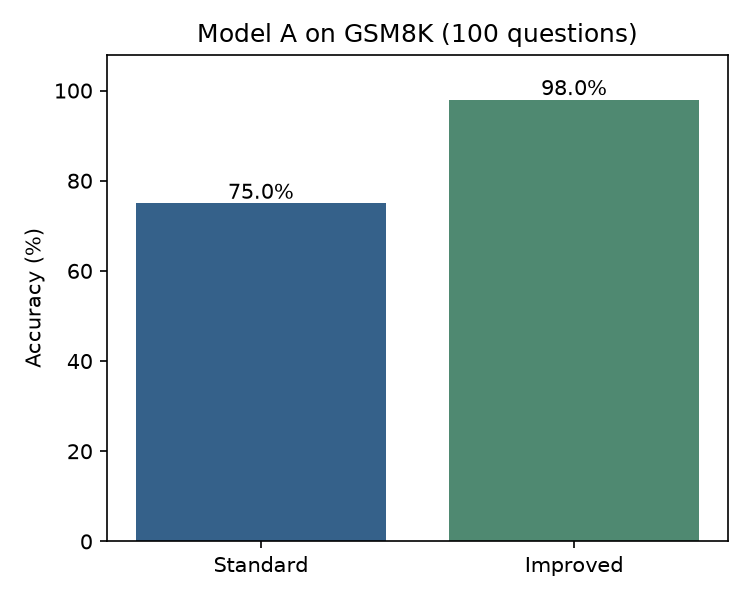
\includegraphics[width=0.65\linewidth]{static/gsm8k_worked_solution.png}
\end{center}

On the same 100 questions, GPT-5.4 with system prompt A improved from
\textbf{75/100} to \textbf{98/100} under the same scoring rule. The new prompt
corrected 23 previously wrong answers and retained all 75 previously correct
answers. For example, in the garden problem there were 10 yellow flowers,
\(10\times1.8=18\) purple flowers, and \((10+18)/4=7\) green flowers.
The new response gave the correct total of 35 rather than 40. Several
instructions changed together, so this run does not isolate their individual
effects.
\end{answer}
